%%%%%%%%%%%%%%%%%%%%%%%%%%%%%%%%%%%%%%%%%
% Journal Article
% LaTeX Template
% Version 1.3 (9/9/13)
%
% This template has been downloaded from:
% http://www.LaTeXTemplates.com
%
% Original author:
% Frits Wenneker (http://www.howtotex.com)
%
% License:
% CC BY-NC-SA 3.0 (http://creativecommons.org/licenses/by-nc-sa/3.0/)
%
%%%%%%%%%%%%%%%%%%%%%%%%%%%%%%%%%%%%%%%%%

%----------------------------------------------------------------------------------------
%	PACKAGES AND OTHER DOCUMENT CONFIGURATIONS
%----------------------------------------------------------------------------------------

\documentclass[twoside]{article}

\usepackage{lipsum} % Package to generate dummy text throughout this template

\usepackage[sc]{mathpazo} % Use the Palatino font
\usepackage[T1]{fontenc} % Use 8-bit encoding that has 256 glyphs
\linespread{1.05} % Line spacing - Palatino needs more space between lines
\usepackage{microtype} % Slightly tweak font spacing for aesthetics

\usepackage[hmarginratio=1:1,top=32mm,columnsep=20pt]{geometry} % Document margins
\usepackage{multicol} % Used for the two-column layout of the document
\usepackage[hang, small,labelfont=bf,up,textfont=it,up]{caption} % Custom captions under/above floats in tables or figures
\usepackage{booktabs} % Horizontal rules in tables
\usepackage{float} % Required for tables and figures in the multi-column environment - they need to be placed in specific locations with the [H] (e.g. \begin{table}[H])
\usepackage{hyperref} % For hyperlinks in the PDF
\usepackage{graphicx}
\usepackage{placeins}
\usepackage{caption}
\usepackage{subcaption}
\usepackage{amsmath}


\usepackage{lettrine} % The lettrine is the first enlarged letter at the beginning of the text
\usepackage{paralist} % Used for the compactitem environment which makes bullet points with less space between them

\usepackage{abstract} % Allows abstract customization
\renewcommand{\abstractnamefont}{\normalfont\bfseries} % Set the "Abstract" text to bold
\renewcommand{\abstracttextfont}{\normalfont\small\itshape} % Set the abstract itself to small italic text

\usepackage{titlesec} % Allows customization of titles
\renewcommand\thesection{\Roman{section}} % Roman numerals for the sections
\renewcommand\thesubsection{\Roman{subsection}} % Roman numerals for subsections
\titleformat{\section}[block]{\large\scshape\centering}{\thesection.}{1em}{} % Change the look of the section titles
\titleformat{\subsection}[block]{\large}{\thesubsection.}{1em}{} % Change the look of the section titles

\usepackage{fancyhdr} % Headers and footers
\pagestyle{fancy} % All pages have headers and footers
\fancyhead{} % Blank out the default header
\fancyfoot{} % Blank out the default footer
\fancyfoot[RO,LE]{\thepage} % Custom footer text

%----------------------------------------------------------------------------------------
%	TITLE SECTION
%----------------------------------------------------------------------------------------

\title{\vspace{-15mm}\fontsize{24pt}{10pt}\selectfont\textbf{A Comparison of Memory Usage Patterns Between Traditional Active Contour Models and Dynamic Programming Snakes}} % Article title

\author{
\large
\textsc{Sumeet Sharma, Praveen Sundar, Nicolas Langley}\\[2mm] % Your name
\normalsize University of California, Los Angeles \\ % Your institution
\vspace{-5mm}
}
\date{}

%----------------------------------------------------------------------------------------

\begin{document}

\maketitle % Insert title

\thispagestyle{fancy} % All pages have headers and footers

%----------------------------------------------------------------------------------------
%	ABSTRACT
%----------------------------------------------------------------------------------------

\begin{abstract}

\noindent 
One of the popular methods used for identifying objects in an image is the active contour model. By adjusting the set of points comprising the snake over time using the image intensity gradients, the snake converges toward some global minimum according to a user-defined energy function. Traditional snakes define a total energy function as a sum of two external and internal energy terms whereas the Dynamic Programming-based snake uses Dynamic Programming to compute an approximate energy minimum. We propose to implement the two types of snakes and compare their memory usages. In our experimental results, the Dynamic Programming snake vastly exceeds the memory usage of the traditional snake counterpart by a solid 20 MB, regardless of how the parameters are set on average. The main drawback of the Dynamic programming snake, despite it's superior speed, is it's difficulty in determining the tuning of the weights for the internal and external energy terms; however, should the Dynamic Programming snake be tuned properly, it's accuracy performs quite well and does it in a shorter amount of time. 

\end{abstract}

%----------------------------------------------------------------------------------------
%	ARTICLE CONTENTS
%----------------------------------------------------------------------------------------

\begin{multicols}{2} % Two-column layout throughout the main article text

\section{Introduction}

\lettrine[nindent=0em,lines=3]{I} mage segmentation is one of the most heavily studied problems in Computer Vision today and has numerous real-world applications. The basic task at hand in the image segmentation task is to create a 2-dimensional closed curve that wraps itself around the perimeter of an object within an image. \par
	In the beginning, the snake is initialized as a generic shape encircling most of the content in the image, oftentimes a circle. For each time step, the points along the snake begin to move inward toward the center of the object, but more specifically toward an object's boundary or edge in the image. This process is accomplished through minimizing an energy function for the entire snake. The energy of a snake is defined as the sum of a snake's internal and external energies. Internal energy of a snake is given as a measurement of the stretching and bending of the snake's structure. On the other hand, external energy is similar to the potential energy of an object based on it's location and relative to another reference point. In our case, the external energy is measured by how far away the image's objects are from the snake's curve in the form of a force, using an image intensity gradient $\nabla I(x,y)$, which is approximated using finite-difference equations for computer vision applications such as image segmentation.


%------------------------------------------------

\section{Traditional Snake}

The traditional snake model is an energy-minimizing spline that accurately localizes nearby edges. This spline is directed according to external constraint forces as well as image forces. The
spline can be viewed as a model:\\
\begin{equation}
  \mathbf{v}(s) = [x(s), y(s)], s \in [0, L]
\end{equation}
where $s$ is the arclength along the snake and $L$ is the total length of the snake\\
A snake has an energy representation that represents the forces that exist on the snake\\
\begin{equation} \label{eq:total_energy}
  E_{total} = \int_{0}^{L} [E_{int}(\mathbf{v}) + \gamma E_{ext}(\mathbf{v})] ds
\end{equation}
This energy function is composed of an energy function for the internal forces, $E_{int}$ and an energy function for the external forces, $E_{ext}$. The internal energy forces are comprised of 
elasticity and rigidity terms.
\begin{equation}
  E_{int}(\mathbf{v}) = \alpha \left| \frac{\partial \mathbf{v}}{ds} \right|^{2} + \beta \left|\frac{\partial^{2}\mathbf{v}}{ds^{2}}\right|^{2}
\end{equation}
This energy function serves as a smoothness constraint on the snake. \\
The external energy function corresponds to the image force and is represented by the negative image gradient.
\begin{equation}
  E_{ext}(\mathbf{v}) = - \nabla I
\end{equation}
The parameters to this model, $\alpha$, $\beta$ and $\gamma$ are weights that penalize the slope, curvature and external forces of the snake, respectively. \\

In the traditional snake model, the spline accurately localizes to nearby edges by minimizing the energy function in ~\ref{eq:total_energy}. The implementation of this minimization
results in two ndependant Euler equations:
\begin{alignat}{2}
  Ax + f_{x}(x,y) &= 0 \\
  Ay + f_{y}(x,y) &= 0
\end{alignat}
where $A$ is a pentadiagonal matrix and $f_{x}, f_{y}$ are the partial derivatives of $E_{ext}$ \\

The above equations can be solved for a timestep $t$ by:
\begin{alignat}{2}
  x_{t} &= (A + \gamma I)^{-1}(x_{t-1} - f_{x}(x_{t-1},y_{t-1})) \\
  y_{t} &= (A + \gamma I)^{-1}(y_{t-1} - f_{y}(x_{t-1},y_{t-1}))
\end{alignat}

Since $A + \gamma I$ is a pentadiagonal banded matrix, it's inverse can be computed using LU-factorization in time $O(n)$

The initial positioning of the traditional snakes on a sample image is:
\FloatBarrier
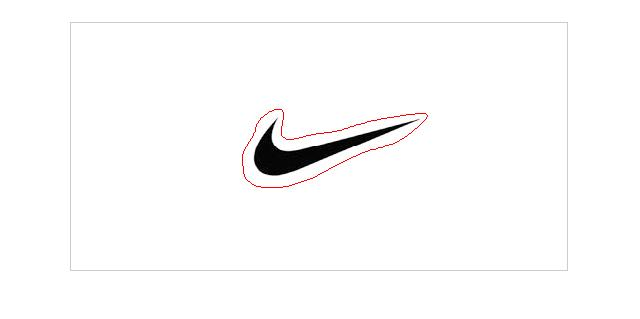
\includegraphics[scale=0.3]{./report_images/snake_preimage.jpg}
\FloatBarrier
The result of 200 iterations of running the snake is:
\FloatBarrier
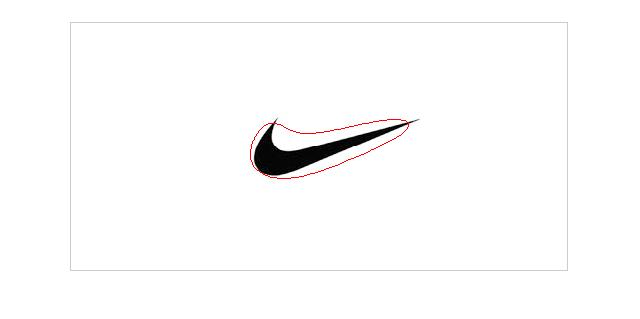
\includegraphics[scale=0.3]{./report_images/snake_postimage.jpg}
\FloatBarrier


%------------------------------------------------

\section{Dynamic Programming Snake}

Unlike the traditional snake model, the Dynamic Programming snake iterates and improves upon a pre-defined number of possible snake vertex positions. During each iteration, the Viterbi algorithm is used to select an optimal snake out of a fixed number of choices for a fixed number of vertex positions. Then once the vertices are selected, a new set of possible snakes are generated according to a custom  importance sampling method to spread vertices to different areas along the snake that are closer to the target object's sharper corners.  To fully connect the snake in a closed loop, the set of points connecting all neighboring pairs of vertices are also considered part of the snake. Since the number of vertices used is variable, a tradeoff must be made in terms of memory usage and accuracy of the final snake positioning. Using more vertices to allow the snake to wrap around corners and sharp edges requires more space for storing computational work and hence slows the algorithm down.
\par  

The algorithm begins with the initialization of constants that define the number of vertices to be used, the length of the set of points along the normal to each vertex, and the spacing of points used as new vertex candidate points along the normals to each vertex. For our project, we initialize vertices to be evenly spaced around a circle of radius as big as possible as to be contained completely within the image's dimensions. Then, for each vertex $v$, the set of normals to each vertex is computed $N(v)$ and has a fixed number of chosen points. Then, the Viterbi algorithm is used to determine the optimal choice of vertex point along each normal from the set $N(v_i)$ for each i. Starting with an arbitrary first vertex $v_1$, the snake's optimal total energy for all vertices up to vertex $i$ is the minimum over all $v_i$ in the set $N(v_i)$ of:
\begin{equation}
E(v_1...v_i) = E(v_1...v_{i-1}) + \alpha E_{ext}(v_i) + \beta E_{int}(v_i)
\end{equation}
To approximate the image gradient, we use for $k,j,p,q \in \{1,2\} $:
\begin{equation}
E^{i}_{external} = \Sigma_i (I(v^{i}_x+k,v^{i}_y+j) - I(v^{i}_x-p,v^{i}_y-q))^2 
\end{equation}
where $I(x,y)$ is the image intensity of a particular pixel.
Then for the internal energy: 
\begin{equation}
E^{i}_{internal} = (v_i - v_{i-1})^2 + (v_{i+1} - 2v_i + v_{i-1})^2 
\end{equation}

Since we have separate energy components for each set of two and three neighboring pixels, the Viterbi algorithm takes a dynamic programming approach to calculating the entire local minimum instead of calculating the total energy for every possible snake in a particular iteration of the DP snake approach. Not using that approach would require enumerating the total energy function $|N|^{|V|}$ times. Instead, we compute partial energy functions for vertices $1...i$ starting from 1. Successive energy calculations and minima only depend on the prior results so by the time $i=|V|$, those energy values will reflect optimal energies of the total snake ending with a particular vertex $v$ in the last $N(v_n)$, where $n=|V|$.
\par
Elaborating on the exact procedure used to perform the importance sampling step in each iteration, the snake is completely connected as a closed shape by interpolating and plotting the points in between consecutive neighboring vertex pairs. Then, for each vertex, two vectors are created using the two line segments leaving each vertex by treating each of the two further endpoints of the segments away from the vertex as the head of each vector and each of the tail points being the vertex itself. Then the angle is determined using the following mathematical fact about vectors: 
\begin{equation}
\theta = cos^{-1}(\frac{v_1 \cdot v_1}{||v_1||_2 ||v_2||_2})
\end{equation}
 Since we want to resample and redistribute vertices evenly but assign vertices to be closer when they're closer to the image portions with sharper edges, we wanted to assign more weight to points closer to vertices that have a smaller angle between that vertex's incoming edges so that vertices in the proximity will be able to detect the hidden object's sharper edges and form a more definitive shape. With the angle in radians, each vertex would be reassigned to another point in the set of points starting from the vertex itself toward the midpoint of the segment in the clockwise direction. These points were discretized to be actual coordinates of pixels. Starting from the midpoint with weight 0, the points leading up to and including the vertex would have weight distributed according to a least-squares fitted exponential curve shifted down by 1 in the range 0 to 1. The following form of the exponential was used to distribute weight up to the vertex point starting from the midpoint:
 \begin{equation}
w = e^{ax}
\end{equation}
This curve was fit to two points using least-squares: $(0,0)$ and $(1,\theta_v)$ where $\theta_v$ is the maximum weight (the angle between $v_1$ and $v_2$ in radians) to be given to re-assigning a vertex to itself. Finally, with the newly chosen weights, every vertex would randomly be replaced by a single randomly chosen surrogate vertex using this distribution of weights. When all the new vertices become chosen, a new round of the entire algorithm repeats a fixed number of pre-defined number of times. 

%------------------------------------------------

\section{Results}

The traditional snakes algorithm was performed over 7 iterations and the memory usage was recorded.
\begin{table}[H]
\caption{Traditional Snakes Memory Usage}
\centering
\begin{tabular}{llr}
\toprule
\cmidrule(r){1-2}
Iteration & Memory Usage (bytes) \\
\midrule
1 & 29.180 \\
2 & 29.180 \\
3 & 29.184 \\
4 & 29.192 \\
5 & 29.196 \\
6 & 29.225 \\
7 & 29.229 \\
\bottomrule
\end{tabular}
\end{table}

The iterations of the traditional snake show that there is no increase in the virtual memory usage between the iterations. The parameters that can be passed to the algorithm are the
$\alpha, \beta, \gamma$ and $\kappa$ values as well as the weights for the different energy functions. \par
The $\alpha$ and $\beta$ parameters are used in the computation of the pentadiagonal matrix $A$. The $\gamma$ and $\kappa$ parameters influence the application of the internal forces in updating
the snake position. However, there is no change in impact with regards to memory usage related to any change in value of these parameters. Additionally, the weight values for the traditional
snake algorithm used in the combination of the different energy functions do not have an effect on the memory usage \\

On the other hand, the Dynamic programming snake displays the following memory usage numbers with respect to varying the parameter number of vertices used in the snake (other parameters such as iteration number, length of the normal, etc, show negligible effects on memory usage so we disregard them and keep them constant).

\begin{table}[H]
\caption{Dynamic Programming Snake Memory Usage}
\centering
\begin{tabular}{llr}
\toprule
\cmidrule(r){1-2}
Number of Vertices & Memory Usage (MB) \\
\midrule
10 & 45.94 \\
15 & 46.26 \\
20 & 46.27 \\
25 & 46.29 \\
30 & 46.30 \\
35 & 46.32 \\
40 & 46.33 \\
\bottomrule
\end{tabular}
\end{table}

From the table, we can see that the memory used by the DP snake increases by approximately 0.015 MB for every 5 more vertices used in the Viterbi calculations and resampling steps.

The images below shows the result of the dynamic programming snake for 10 iterations.

The vertex points obtained after applying the viterbi algorithm for 10 vertices is:
\FloatBarrier
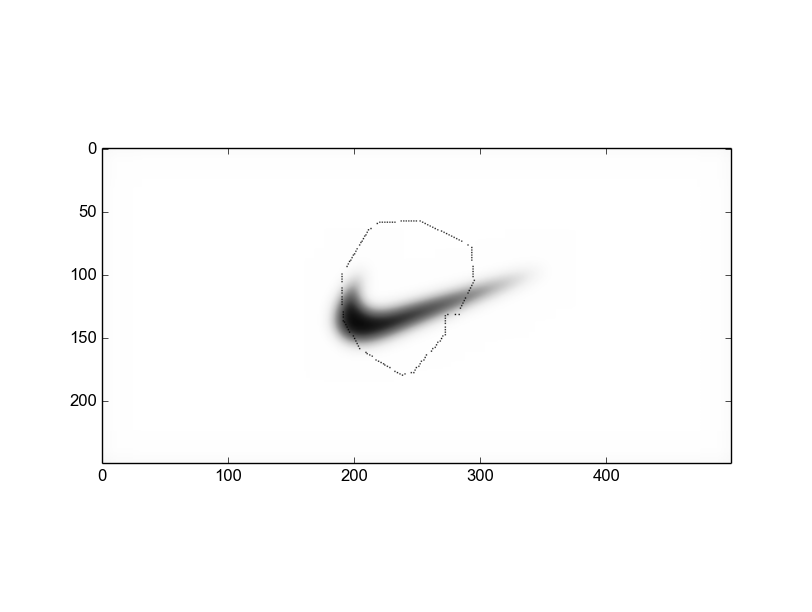
\includegraphics[scale=0.3]{./report_images/viterbi_10vertices.png}
\FloatBarrier

The vertex points obtained after applying the viterbi algorithm for 45 vertices is:
\FloatBarrier
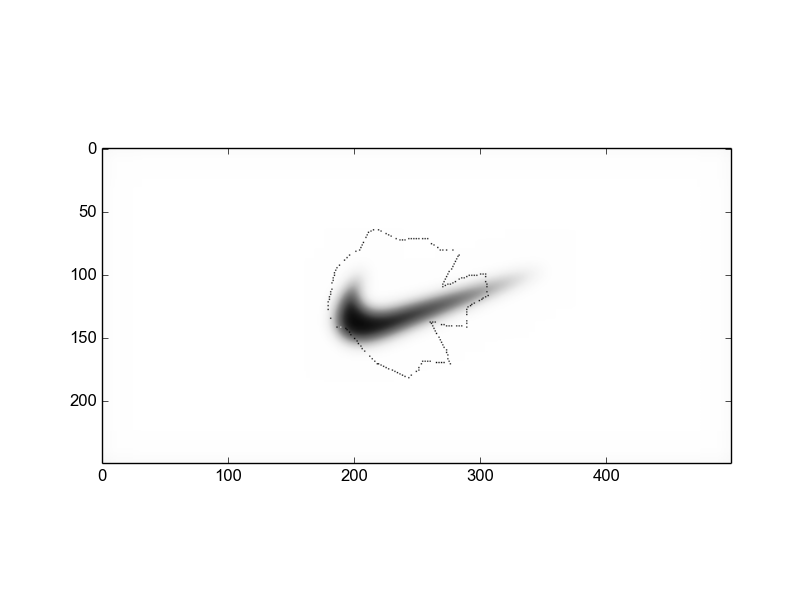
\includegraphics[scale=0.3]{./report_images/viterbi_45vertices.png}
\FloatBarrier

%------------------------------------------------

\section{Discussion}

Given the steady linear increase in memory usage by the Dynamic Programming snake, satisfactory results for image segmentation can be obtained quickly using this method with the small cost of about 20 more MB than that of the original snake. Using more than 40 vertices poses negligible extra memory costs and, as shown in the diagrams, dramatically improves the snake's convergence ability.

%----------------------------------------------------------------------------------------
%	REFERENCE LIST
%----------------------------------------------------------------------------------------

\begin{thebibliography}{99} % Bibliography - this is intentionally simple in this template

\bibitem[Mishra, Fieguth and Clausi, 2008]
aMishra, A., Fieguth, P. and Clausi, D. (2008).
\newblock Accurate boundary localization using dynamic programming on snake
\newblock {\em Proc. Canadian Conf. Computer Robot Vision}, 261--268.

\bibitem[Kass, Witkin and Terzopoulos, 1988]
aKass, M., Witkin, A. and Terzopoulos, D. (1988).
\newblock Snakes: Active Contour Models 
\newblock {\em International journal of computer vision 1.4}, 321--331.
 
\end{thebibliography}

%----------------------------------------------------------------------------------------

\end{multicols}

\end{document}
